\documentclass[journal,12pt,twocolumn]{IEEEtran}
\usepackage{cite}
\usepackage{amsmath,amssymb,amsfonts,amsthm}
\usepackage{algorithmic}
\usepackage{graphicx}
\usepackage{textcomp}
\usepackage{xcolor}
\usepackage{txfonts}
\usepackage{listings}
\usepackage{enumitem}
\usepackage{mathtools}
\usepackage{gensymb}
\usepackage{comment}
\usepackage[breaklinks=true]{hyperref}
\usepackage{tkz-euclide} 
\usepackage{textgreek}                       
\usepackage{circuitikz}
\usepackage{pgfplots}                            
\usepackage[latin1]{inputenc}                                
\usepackage{color}                                            
\usepackage{array}                                            
\usepackage{longtable}                                       
\usepackage{calc}                                             
\usepackage{multirow}                                         
\usepackage{hhline}                                           
\usepackage{ifthen}                                           
\usepackage{lscape}

\newtheorem{theorem}{Theorem}[section]
\newtheorem{problem}{Problem}
\newtheorem{proposition}{Proposition}[section]
\newtheorem{lemma}{Lemma}[section]
\newtheorem{corollary}[theorem]{Corollary}
\newtheorem{example}{Example}[section]
\newtheorem{definition}[problem]{Definition}
\newcommand{\BEQA}{\begin{eqnarray}}
\newcommand{\EEQA}{\end{eqnarray}}
\newcommand{\define}{\stackrel{\triangle}{=}}
\theoremstyle{remark}
\newtheorem{rem}{Remark}

\begin{document}

\bibliographystyle{IEEEtran}
\vspace{3cm}

\title{NCERT 11.9.2  Q7}
\author{EE23BTECH11204 - Ashley Ann Benoy$^{*}$}% <-this % stops a space
\maketitle
\newpage
\bigskip

\renewcommand{\thefigure}{\theenumi}
\renewcommand{\thetable}{\theenumi}

\bibliographystyle{IEEEtran}

\textbf{Question: Find the sum of n terms of the A.P. whose kth term is \(5k + 1\).}

\textbf{Solution:}
\textbf{
\begin{table}[htbp]
\centering
\caption{Given Data}
\label{tab:data}
\begin{tabular}{|c|c|c|}
\hline
\textbf{Symbol} & \textbf{Value} & \textbf{Parameter} \\
\hline
\(x(0)\) & \(1 \) & First Term \\
\hline
\(x(k)\) & \(5k + 1 \) & kth Term \\
\hline
\(d\) & \(5 \) & Common Difference \\
\hline
\(S(n)\) & \(?\) & Sum of \(N\) terms \\
\hline
\end{tabular}
\end{table}
}


Apply the Z-transform to \( x(n) \):
\begin{align}
X(z) = \frac{5z^{-1}}{(1 - z^{-1})^2} + \frac{1}{(1 - z^{-1})}
\quad |z|>1
\end{align}

Sum of First \( n+1 \) Terms:
Express the sum of the first \( n+1 \) terms (\( y(n) \)) in terms of \( x(n) \) using convolution:
\begin{align}
y(n) = x(n) * u(n)
\end{align}

Applying Z transform on both sides:
\begin{align}
    Y(z) &= X(z)U(z)\\
    &=\frac{1}{(1-z^{-1})^2} + \frac{5z^{-1}}{(1-z^{-1})^3}
\end{align}

Given expressions:
\begin{align}
    X_1(z) &= \frac{1}{{(1 - z^{-1})^2}} \\
    X_2(z) &= \frac{5z^{-1}}{{(1 - z^{-1})^3}} \label{eq:x2z}
\end{align}

Using z-transform pairs:

1.\( \mathcal{Z}\{n u[n]\} = \frac{z}{(z-1)^2} \) with ROC \( |z| > 1 \)
\\\\
2.\( \mathcal{Z}\{n(n-1) u[n]\} = \frac{2z}{(z-1)^3} \) with ROC \( |z| > 1 \)
\\\\

Rewriting the expression:
\begin{align}
&\frac{1}{(1 - z^{-1})^2} + \frac{5}{2} \cdot \frac{2z^{-1}}{(1 - z^{-1})^3} 
\end{align}
\\
\begin{align}
&= \mathcal{Z}\{n u[n]\} + \frac{5}{2} \mathcal{Z}\{n(n-1) u[n]\}
\end{align}
\\
Therefore, the inverse z-transform of the sum is:
\begin{align}
y[n] = n u[n] + \frac{5}{2} n(n-1) u[n]
\end{align}

The stem plot is given as
\begin{figure}[h]
  \centering
  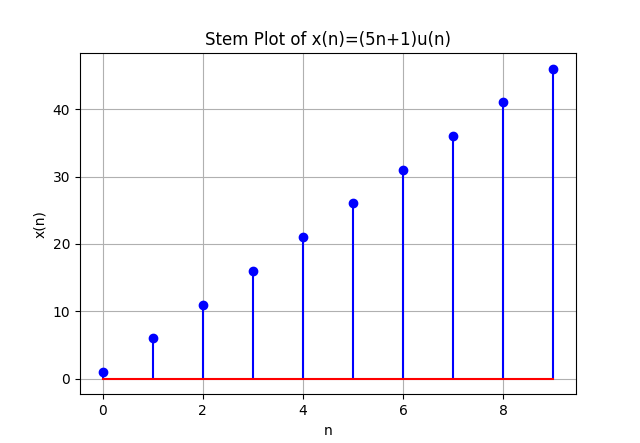
\includegraphics[width=0.6\textwidth]{figs/stem.png}
  \label{fig:Stem_Plot}
\end{figure}
\end{document}
